\documentclass[aspectratio=169]{beamer}
% Add slides directory to search path for Dartmouth theme
\makeatletter
\def\input@path{{../}}
\makeatother
\usetheme{Dartmouth}
\usepackage{booktabs}
\usepackage{listings}
\usepackage{tikz}
\usetikzlibrary{arrows.meta,positioning,shapes,decorations.pathreplacing,calc}
\usepackage{hyperref}
\usepackage{xcolor}
\usepackage{graphicx}
\usepackage{fontspec}
\usepackage{tcolorbox}
\usepackage{amsmath}
\usepackage{amssymb}
\usepackage{pgfplots}
\pgfplotsset{compat=1.18}

% Color scheme
\definecolor{darkblue}{RGB}{0,82,155}
\definecolor{lightblue}{RGB}{100,181,246}
\definecolor{darkgreen}{RGB}{46,125,50}
\definecolor{orange}{RGB}{255,152,0}
\definecolor{purple}{RGB}{142,36,170}
\definecolor{thinkbox}{RGB}{255,245,220}
\definecolor{discussbox}{RGB}{230,240,255}

\setbeamercolor{progress bar}{fg=lightblue,bg=lightblue!30}

% Code listing settings
\lstset{
    basicstyle=\ttfamily\small,
    breaklines=true,
    frame=single,
    backgroundcolor=\color{gray!10},
    keywordstyle=\color{darkblue}\bfseries,
    commentstyle=\color{darkgreen}\itshape,
    stringstyle=\color{orange},
    showstringspaces=false,
    language=Python
}

% Custom boxes
\newtcolorbox{thinkaboutit}{
    colback=thinkbox,
    colframe=orange,
    title=💭 Think about it!,
    fonttitle=\bfseries
}

\newtcolorbox{discussion}{
    colback=discussbox,
    colframe=blue,
    title=💬 Discussion,
    fonttitle=\bfseries
}

\title{Lecture 19: Scaling Up to GPT-3 and Beyond}
\subtitle{The Era of Few-Shot Learning 🚀}
\author{Models of Language and Conversation}
\institute{Dr. Jeremy R. Manning}
\date{Week 7}

\begin{document}

% Title slide
\begin{frame}
    \titlepage
\end{frame}

% Table of contents
\begin{frame}{Today's Journey 🗺️}
    \tableofcontents
\end{frame}

\section{From GPT to GPT-2}

\begin{frame}[shrink=10]{GPT-2: The Unexpected Leap 📈}
    \begin{discussion}
        What happens when we scale up GPT by 10x?
    \end{discussion}

    \vspace{0.3cm}

    \begin{columns}[T]
        \begin{column}{0.48\textwidth}
            \textbf{GPT (2018):}
            \begin{itemize}\setlength{\itemsep}{0pt}
                \item 117M parameters
                \item 5B tokens training
                \item BooksCorpus
                \item Requires fine-tuning
            \end{itemize}
        \end{column}

        \begin{column}{0.48\textwidth}
            \textbf{GPT-2 (2019):}
            \begin{itemize}\setlength{\itemsep}{0pt}
                \item 1.5B parameters (13x larger)
                \item 40GB text (8x more data)
                \item WebText dataset
                \item \textbf{No fine-tuning needed!}
            \end{itemize}
        \end{column}
    \end{columns}

    \vspace{0.3cm}

    \begin{alertblock}{Key Claim}
        "Language models are unsupervised multitask learners"
    \end{alertblock}

    \vspace{0.3cm}

    \small
    \textit{Reference: Radford et al. (2019) - "Language Models are Unsupervised Multitask Learners"}
\end{frame}

\begin{frame}[shrink=10]{The WebText Dataset 🌐}
\small
    \textbf{How GPT-2 was trained:}

    \vspace{0.3cm}

    \begin{block}{WebText Creation}
        \begin{enumerate}\setlength{\itemsep}{0pt}
            \item Scrape all outbound links from Reddit with ≥3 karma
            \item Filter for quality and diversity
            \item Remove Wikipedia (to avoid test set contamination)
            \item Result: 40GB of text, 8 million documents
        \end{enumerate}
    \end{block}

    \vspace{0.3cm}

    \textbf{Why Reddit links?}
    \begin{itemize}\setlength{\itemsep}{0pt}
        \item 👍 Community curation (karma = quality signal)
        \item 📚 Diverse topics and writing styles
        \item 🌍 Web-scale variety
        \item 🎯 Human-filtered content
    \end{itemize}

    \vspace{0.3cm}

    \begin{thinkaboutit}
        This introduced a new paradigm: curated web scraping as training data!
    \end{thinkaboutit}
\end{frame}

\begin{frame}{GPT-2 Model Sizes 📊}
    \textbf{Four model sizes released progressively:}

    \vspace{0.3cm}

    \begin{table}
        \begin{tabular}{lccc}
            \toprule
            \textbf{Model} & \textbf{Parameters} & \textbf{Layers} & \textbf{d\_model} \\
            \midrule
            Small & 117M & 12 & 768 \\
            Medium & 345M & 24 & 1024 \\
            Large & 762M & 36 & 1280 \\
            \textbf{XL} & \textbf{1.5B} & \textbf{48} & \textbf{1600} \\
            \bottomrule
        \end{tabular}
    \end{table}

    \vspace{0.3cm}

    \textbf{Staged release strategy:}
    \begin{itemize}\setlength{\itemsep}{0pt}
        \item Feb 2019: Released small model (117M)
        \item May 2019: Medium model (345M)
        \item Aug 2019: Large model (762M)
        \item Nov 2019: Full model (1.5B)
        \item Concerns about misuse led to gradual release
    \end{itemize}
\end{frame}

\begin{frame}{Zero-Shot Task Transfer 🎯}
    \textbf{The surprising finding: GPT-2 can perform tasks without fine-tuning!}

    \vspace{0.3cm}

    \begin{block}{Zero-Shot Prompting}
        Instead of fine-tuning, just format the task as text:

        \vspace{0.3cm}

        \textbf{Translation:}
        \texttt{English: I love machine learning\\
        French: }

        \vspace{0.3cm}

        \textbf{Question Answering:}
        \texttt{Answer the question:\\
        Q: What is the capital of France?\\
        A: }

        \vspace{0.3cm}

        \textbf{Summarization:}
        \texttt{[Article text]\\
        TL;DR: }
    \end{block}

    \vspace{0.3cm}

    \begin{alertblock}{No task-specific training needed!}
    \end{alertblock}
\end{frame}

\begin{frame}[shrink=10]{GPT-2 Performance 📈}
    \textbf{Zero-shot results on various benchmarks:}

    \vspace{0.3cm}

    \begin{table}
        \small
        \begin{tabular}{lcccc}
            \toprule
            \textbf{Task} & \textbf{Metric} & \textbf{Fine-tuned SOTA} & \textbf{GPT-2 Zero-shot} \\
            \midrule
            Reading Comp. & F1 & 89.3 & 55.0 \\
            Translation (En→Fr) & BLEU & 45.6 & 11.5 \\
            Summarization & ROUGE & 40.2 & 29.3 \\
            Question Answering & Accuracy & 89.4 & 63.1 \\
            \bottomrule
        \end{tabular}
    \end{table}

    \vspace{0.3cm}

    \begin{columns}[T]
        \begin{column}{0.48\textwidth}
            \textbf{✅ Promising:}
            \begin{itemize}\setlength{\itemsep}{0pt}
                \item Works without fine-tuning
                \item Generalizes across tasks
                \item Improves with scale
            \end{itemize}
        \end{column}

        \begin{column}{0.48\textwidth}
            \textbf{⚠️ Limitations:}
            \begin{itemize}\setlength{\itemsep}{0pt}
                \item Still behind fine-tuned models
                \item Inconsistent quality
                \item Hard to control
            \end{itemize}
        \end{column}
    \end{columns}
\end{frame}

\begin{frame}{Text Generation Quality 📝}
    \begin{block}{GPT-2 Generated Text Sample}
        \small
        \textbf{Prompt:} "In a shocking finding, scientist discovered a herd of unicorns living in a remote, previously unexplored valley, in the Andes Mountains."

        \vspace{0.3cm}

        \textbf{GPT-2 continues:}
        "Even more surprising to the researchers was the fact that the unicorns spoke perfect English. The scientist named the population, after their distinctive horn, Ovid's Unicorn. These four-horned, silver-white unicorns were previously unknown to science..."
    \end{block}

    \vspace{0.3cm}

    \textbf{Observations:}
    \begin{itemize}\setlength{\itemsep}{0pt}
        \item ✅ Coherent and fluent
        \item ✅ Maintains context and style
        \item ⚠️ Completely fabricated "facts"
        \item ⚠️ No grounding in reality
    \end{itemize}

    \vspace{0.3cm}

    \begin{thinkaboutit}
        The model is \textit{too good} at generating plausible-sounding nonsense!
    \end{thinkaboutit}
\end{frame}

\section{GPT-3: Scale Changes Everything}

\begin{frame}{GPT-3: The 175B Parameter Model 🌟}
    \begin{discussion}
        What happens when we scale up another 100x?
    \end{discussion}

    \vspace{0.3cm}

    \begin{center}
        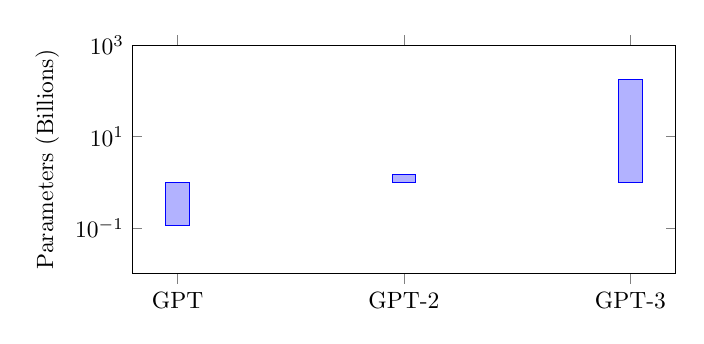
\begin{tikzpicture}[scale=0.85]
            \begin{axis}[
                ybar,
                width=0.8\textwidth,
                height=5cm,
                ylabel={Parameters (Billions)},
                symbolic x coords={GPT, GPT-2, GPT-3},
                xtick=data,
                ymode=log,
                log basis y=10,
                ylabel near ticks,
                ymin=0.01,
                ymax=1000,
            ]
            \addplot coordinates {
                (GPT, 0.117)
                (GPT-2, 1.5)
                (GPT-3, 175)
            };
            \end{axis}
        \end{tikzpicture}
    \end{center}

    \vspace{0.3cm}

    \small
    \textit{Reference: Brown et al. (2020) - "Language Models are Few-Shot Learners"}
\end{frame}

\begin{frame}{GPT-3 Model Specifications 📊}
    \begin{table}
        \begin{tabular}{lc}
            \toprule
            \textbf{Specification} & \textbf{Value} \\
            \midrule
            Parameters & 175 billion \\
            Layers & 96 \\
            Hidden size (d\_model) & 12,288 \\
            Attention heads & 96 \\
            Context window & 2048 tokens \\
            Training tokens & 300 billion \\
            Training data & 570GB (filtered) \\
            Training compute & ~3640 petaflop-days \\
            Training cost & \textasciitilde\$4.6M \\
            \bottomrule
        \end{tabular}
    \end{table}

    \vspace{0.3cm}

    \begin{alertblock}{Scale}
        GPT-3 is so large it has never been fully fine-tuned—only used via API!
    \end{alertblock}
\end{frame}

\begin{frame}{GPT-3 Training Data 📚}
    \textbf{Training corpus composition:}

    \vspace{0.3cm}

    \begin{table}
        \small
        \begin{tabular}{lcc}
            \toprule
            \textbf{Dataset} & \textbf{Quantity} & \textbf{Weight in training} \\
            \midrule
            Common Crawl (filtered) & 410B tokens & 60\% \\
            WebText2 & 19B tokens & 22\% \\
            Books1 & 12B tokens & 8\% \\
            Books2 & 55B tokens & 8\% \\
            Wikipedia & 3B tokens & 3\% \\
            \bottomrule
        \end{tabular}
    \end{table}

    \vspace{0.3cm}

    \textbf{Key differences from GPT-2:}
    \begin{itemize}\setlength{\itemsep}{0pt}
        \item Much larger and more diverse
        \item Includes Common Crawl (with quality filtering)
        \item Multiple passes over high-quality data
        \item Carefully balanced mixture
    \end{itemize}
\end{frame}

\begin{frame}[shrink=10]{Few-Shot Learning 🎓}
\small
    \textbf{GPT-3's key capability: In-context learning}

    \vspace{0.3cm}

    \begin{block}{Learning Paradigms}
        \begin{enumerate}\setlength{\itemsep}{0pt}
            \item \textbf{Zero-shot}: Task description only
            \begin{itemize}\setlength{\itemsep}{0pt}
                \item \texttt{Translate to French: I love AI →}
            \end{itemize}

            \vspace{0.3cm}

            \item \textbf{One-shot}: One example
            \begin{itemize}\setlength{\itemsep}{0pt}
                \item \texttt{sea otter → loutre de mer}
                \item \texttt{I love AI →}
            \end{itemize}

            \vspace{0.3cm}

            \item \textbf{Few-shot}: Multiple examples (typically 10-100)
            \begin{itemize}\setlength{\itemsep}{0pt}
                \item \texttt{dog → chien}
                \item \texttt{cat → chat}
                \item \texttt{bird → oiseau}
                \item \texttt{I love AI →}
            \end{itemize}
        \end{enumerate}
    \end{block}

    \vspace{0.3cm}

    \textbf{No gradient updates! Just prompt engineering.}
\end{frame}

\begin{frame}{In-Context Learning Mechanism 🧠}
    \begin{center}
        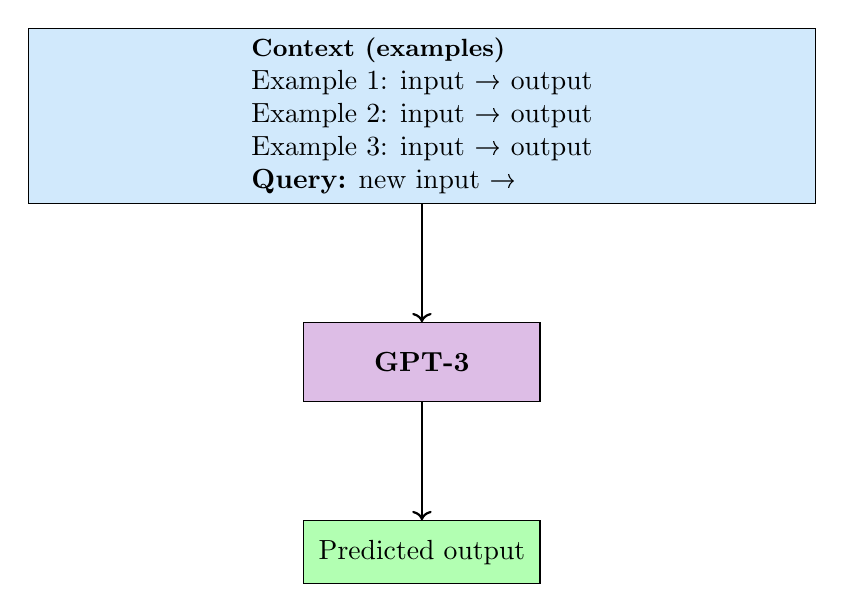
\begin{tikzpicture}[scale=0.85,node distance=1.5cm]
            % Context window
            \node[draw, rectangle, fill=lightblue!30, minimum width=10cm, minimum height=1.5cm, align=left] (context) {
                \small
                \textbf{Context (examples)} \\
                Example 1: input → output \\
                Example 2: input → output \\
                Example 3: input → output \\
                \textbf{Query:} new input →
            };

            % GPT-3
            \node[draw, rectangle, fill=purple!30, minimum width=3cm, minimum height=1cm, below=of context] (gpt3) {
                \textbf{GPT-3}
            };

            % Output
            \node[draw, rectangle, fill=green!30, minimum width=3cm, minimum height=0.8cm, below=of gpt3] (output) {
                Predicted output
            };

            % Arrows
            \draw[->, thick] (context) -- (gpt3);
            \draw[->, thick] (gpt3) -- (output);
        \end{tikzpicture}
    \end{center}

    \vspace{0.3cm}

    \textbf{How does it work?}
    \begin{itemize}\setlength{\itemsep}{0pt}
        \item Model recognizes pattern in examples
        \item Continues the pattern for new input
        \item No weight updates—pure inference!
        \item "Learning" happens at inference time
    \end{itemize}
\end{frame}

\begin{frame}{GPT-3 Performance Across Tasks 📊}
    \begin{center}
        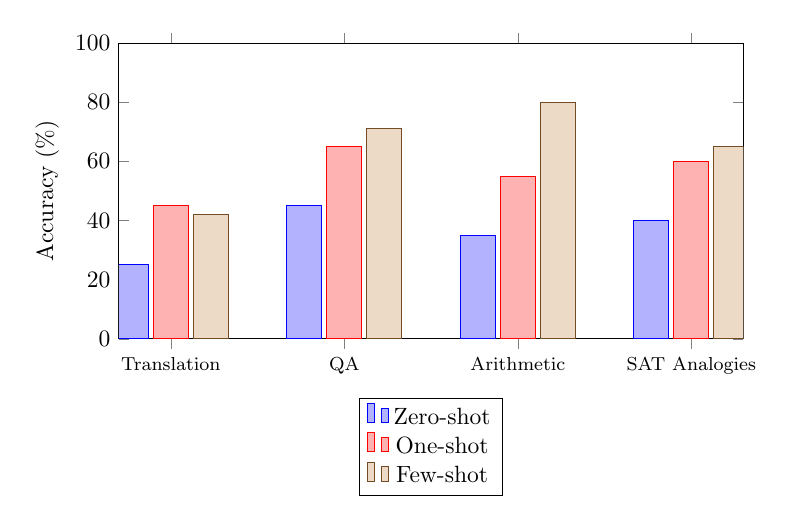
\begin{tikzpicture}[scale=0.85]
            \begin{axis}[
                ybar,
                width=0.9\textwidth,
                height=6cm,
                ylabel={Accuracy (\%)},
                symbolic x coords={Translation, QA, Arithmetic, SAT Analogies},
                xtick=data,
                legend style={at={(0.5,-0.2)},anchor=north},
                ylabel near ticks,
                ymin=0,
                ymax=100,
                bar width=15pt,
                x tick label style={font=\footnotesize},
            ]
            \addplot coordinates {
                (Translation, 25)
                (QA, 45)
                (Arithmetic, 35)
                (SAT Analogies, 40)
            };
            \addplot coordinates {
                (Translation, 45)
                (QA, 65)
                (Arithmetic, 55)
                (SAT Analogies, 60)
            };
            \addplot coordinates {
                (Translation, 42)
                (QA, 71)
                (Arithmetic, 80)
                (SAT Analogies, 65)
            };
            \legend{Zero-shot, One-shot, Few-shot}
            \end{axis}
        \end{tikzpicture}
    \end{center}

    \vspace{0.3cm}

    \textbf{Key observation: More examples = better performance}
\end{frame}

\begin{frame}[shrink=10]{GPT-3's Emergent Abilities ✨}
    \begin{discussion}
        What can GPT-3 do that smaller models can't?
    \end{discussion}

    \vspace{0.3cm}

    \textbf{Emergent capabilities:}
    \begin{itemize}\setlength{\itemsep}{0pt}
        \item 🧮 \textbf{Arithmetic}: 2-3 digit addition/subtraction
        \item 💭 \textbf{Reasoning}: Simple logical deduction
        \item 🎨 \textbf{Code generation}: Write simple programs
        \item 🌍 \textbf{Knowledge synthesis}: Combine facts
        \item 📝 \textbf{Style transfer}: Mimic writing styles
        \item 🎯 \textbf{Task composition}: Multi-step procedures
    \end{itemize}

    \vspace{0.3cm}

    \begin{alertblock}{Scaling Hypothesis}
        These abilities weren't explicitly trained—they \textit{emerged} from scale!
    \end{alertblock}

    \vspace{0.3cm}

    \small
    \textit{Reference: Wei et al. (2022) - "Emergent Abilities of Large Language Models"}
\end{frame}

\section{Scaling Laws}

\begin{frame}[shrink=10]{The Scaling Laws Hypothesis 📈}
\small
    \begin{block}{Kaplan et al. (2020) - "Scaling Laws for Neural Language Models"}
        Model performance scales as a \textbf{power law} with:
        \begin{itemize}\setlength{\itemsep}{0pt}
            \item Model size (parameters)
            \item Dataset size (tokens)
            \item Compute (FLOPs)
        \end{itemize}
    \end{block}

    \vspace{0.3cm}

    \textbf{Key findings:}
    \begin{enumerate}\setlength{\itemsep}{0pt}
        \item Performance depends strongly on scale
        \item Very weak dependence on model shape (depth vs width)
        \item Smooth, predictable improvements
        \item Optimal compute allocation: Grow model and data together
    \end{enumerate}

    \vspace{0.3cm}

    \begin{thinkaboutit}
        If scaling laws hold, we can predict future model performance!
    \end{thinkaboutit}
\end{frame}

\begin{frame}{The Scaling Law Formula ⚖️}
    \textbf{Loss as a function of scale:}

    \vspace{0.3cm}

    $$L(N) = \left(\frac{N_c}{N}\right)^{\alpha_N}$$

    where:
    \begin{itemize}\setlength{\itemsep}{0pt}
        \item $L$ = Cross-entropy loss
        \item $N$ = Number of parameters
        \item $N_c$ = Scaling constant
        \item $\alpha_N \approx 0.076$ (empirically determined)
    \end{itemize}

    \vspace{0.3cm}

    \begin{center}
        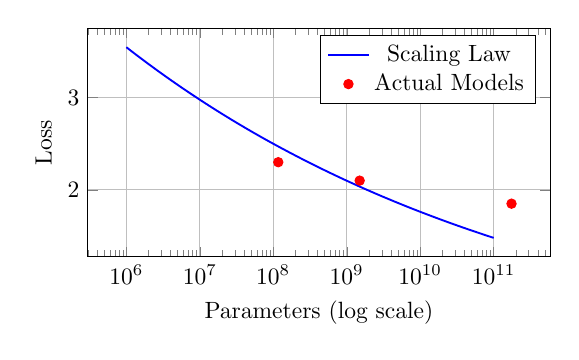
\begin{tikzpicture}[scale=0.85]
            \begin{axis}[
                width=0.7\textwidth,
                height=5cm,
                xlabel={Parameters (log scale)},
                ylabel={Loss},
                xmode=log,
                grid=major,
                legend pos=north east,
            ]
            \addplot[blue, thick, domain=1e6:1e11, samples=50] {2.5*(1e8/x)^0.076};
            \addlegendentry{Scaling Law}
            \addplot[red, only marks, mark=*, mark size=2pt] coordinates {
                (1.17e8, 2.3)
                (1.5e9, 2.1)
                (1.75e11, 1.85)
            };
            \addlegendentry{Actual Models}
            \end{axis}
        \end{tikzpicture}
    \end{center}
\end{frame}

\begin{frame}[shrink=10]{Implications of Scaling Laws 🎯}
    \begin{columns}[T]
        \begin{column}{0.48\textwidth}
            \textbf{✅ Good news:}
            \begin{itemize}\setlength{\itemsep}{0pt}
                \item Predictable improvements
                \item Clear path to better models
                \item Can plan compute budgets
                \item Smooth progress curve
            \end{itemize}
        \end{column}

        \begin{column}{0.48\textwidth}
            \textbf{⚠️ Challenges:}
            \begin{itemize}\setlength{\itemsep}{0pt}
                \item Diminishing returns
                \item Exponential cost increase
                \item Hardware limitations
                \item Environmental impact
            \end{itemize}
        \end{column}
    \end{columns}

    \vspace{0.5cm}

    \begin{alertblock}{The Scaling Question}
        To improve loss by 0.1: \\
        $N_{new} = N_{old} \times \left(\frac{L_{old}}{L_{new}}\right)^{1/\alpha} \approx N_{old} \times 10^{13}$

        \vspace{0.3cm}

        Massive compute increase for small improvements!
    \end{alertblock}
\end{frame}

\begin{frame}{Chinchilla Scaling Laws 🐭}
    \begin{block}{Hoffmann et al. (2022) - "Training Compute-Optimal Large Language Models"}
        Previous models were over-parameterized and under-trained!
    \end{block}

    \vspace{0.3cm}

    \textbf{Key insight:}
    \begin{itemize}\setlength{\itemsep}{0pt}
        \item For a given compute budget, should balance model size and data
        \item \textbf{Optimal ratio}: 20 tokens per parameter
        \item GPT-3 (175B params, 300B tokens): Under-trained!
        \item Chinchilla (70B params, 1.4T tokens): Better performance
    \end{itemize}

    \vspace{0.3cm}

    \begin{thinkaboutit}
        Instead of making models bigger, train longer on more data!
    \end{thinkaboutit}

    \vspace{0.3cm}

    \small
    \textit{This influenced Llama 2, GPT-4, and other modern models}
\end{frame}

\section{From GPT-3 to ChatGPT}

\begin{frame}[shrink=5]{The Path to ChatGPT 🤖}
    \begin{center}
        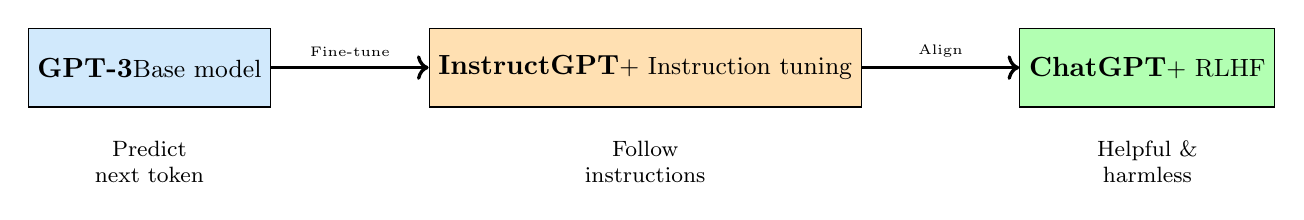
\begin{tikzpicture}[scale=0.85,node distance=2cm]
            % GPT-3
            \node[draw, rectangle, fill=lightblue!30, minimum width=3cm, minimum height=1cm] (gpt3) {
                \textbf{GPT-3}\\
                \small Base model
            };

            % InstructGPT
            \node[draw, rectangle, fill=orange!30, minimum width=3cm, minimum height=1cm, right=of gpt3] (instruct) {
                \textbf{InstructGPT}\\
                \small + Instruction tuning
            };

            % ChatGPT
            \node[draw, rectangle, fill=green!30, minimum width=3cm, minimum height=1cm, right=of instruct] (chat) {
                \textbf{ChatGPT}\\
                \small + RLHF
            };

            % Arrows
            \draw[->, very thick] (gpt3) -- (instruct) node[midway, above, font=\tiny] {Fine-tune};
            \draw[->, very thick] (instruct) -- (chat) node[midway, above, font=\tiny] {Align};

            % Labels
            \node[below=0.3cm of gpt3, align=center, font=\footnotesize] {Predict\\next token};
            \node[below=0.3cm of instruct, align=center, font=\footnotesize] {Follow\\instructions};
            \node[below=0.3cm of chat, align=center, font=\footnotesize] {Helpful \&\\harmless};
        \end{tikzpicture}
    \end{center}

    \vspace{0.3cm}

    \textbf{Three key innovations:}
    \begin{enumerate}\setlength{\itemsep}{0pt}
        \item \textbf{Instruction tuning}: Train to follow instructions
        \item \textbf{RLHF}: Reinforcement Learning from Human Feedback
        \item \textbf{Safety guardrails}: Reduce harmful outputs
    \end{enumerate}
\end{frame}

\begin{frame}[shrink=10]{Instruction Tuning 📋}
\small
    \begin{block}{What is Instruction Tuning?}
        Fine-tune the model on (instruction, response) pairs to make it better at following user commands.
    \end{block}

    \vspace{0.3cm}

    \textbf{Training examples:}
    \begin{itemize}\setlength{\itemsep}{0pt}
        \item \textit{"Explain quantum computing to a 5-year-old"} → [explanation]
        \item \textit{"Write a Python function to sort a list"} → [code]
        \item \textit{"Summarize this article in 3 sentences"} → [summary]
    \end{itemize}

    \vspace{0.3cm}

    \begin{columns}[T]
        \begin{column}{0.48\textwidth}
            \textbf{Before (GPT-3):}
            \begin{itemize}\setlength{\itemsep}{0pt}
                \item Continues the text
                \item Often misunderstands intent
                \item Needs careful prompting
            \end{itemize}
        \end{column}

        \begin{column}{0.48\textwidth}
            \textbf{After (InstructGPT):}
            \begin{itemize}\setlength{\itemsep}{0pt}
                \item Follows instructions
                \item Clear, helpful responses
                \item More controllable
            \end{itemize}
        \end{column}
    \end{columns}
\end{frame}

\begin{frame}{RLHF: Reinforcement Learning from Human Feedback 👍}
    \begin{center}
        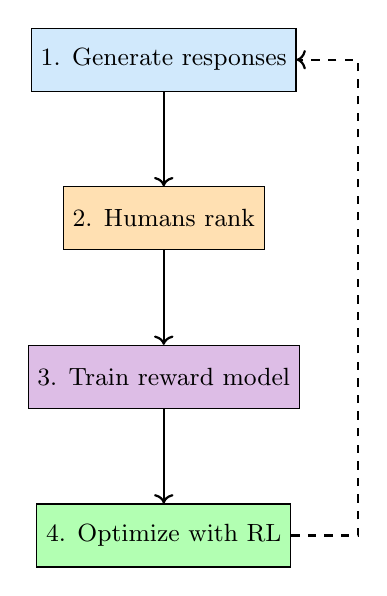
\begin{tikzpicture}[scale=0.85,node distance=1.2cm]
            % Step 1
            \node[draw, rectangle, fill=lightblue!30, minimum width=2.5cm, minimum height=0.8cm] (step1) {
                \small 1. Generate responses
            };

            % Step 2
            \node[draw, rectangle, fill=orange!30, minimum width=2.5cm, minimum height=0.8cm, below=of step1] (step2) {
                \small 2. Humans rank
            };

            % Step 3
            \node[draw, rectangle, fill=purple!30, minimum width=2.5cm, minimum height=0.8cm, below=of step2] (step3) {
                \small 3. Train reward model
            };

            % Step 4
            \node[draw, rectangle, fill=green!30, minimum width=2.5cm, minimum height=0.8cm, below=of step3] (step4) {
                \small 4. Optimize with RL
            };

            % Arrows
            \draw[->, thick] (step1) -- (step2);
            \draw[->, thick] (step2) -- (step3);
            \draw[->, thick] (step3) -- (step4);
            \draw[->, thick, dashed] (step4.east) -- ++(1,0) |- (step1.east);
        \end{tikzpicture}
    \end{center}

    \vspace{0.3cm}

    \textbf{Why RLHF?}
    \begin{itemize}\setlength{\itemsep}{0pt}
        \item Hard to write perfect instruction examples
        \item Easier to compare: "Which response is better?"
        \item Learns subtle preferences (tone, safety, helpfulness)
        \item Aligns model with human values
    \end{itemize}
\end{frame}

\begin{frame}[shrink=10]{ChatGPT's Impact 🌍}
    \textbf{Launched: November 30, 2022}

    \vspace{0.3cm}

    \textbf{Growth:}
    \begin{itemize}\setlength{\itemsep}{0pt}
        \item 1 million users in 5 days
        \item 100 million users in 2 months
        \item Fastest-growing consumer application ever
    \end{itemize}

    \vspace{0.3cm}

    \textbf{Why so successful?}
    \begin{itemize}\setlength{\itemsep}{0pt}
        \item ✅ Easy to use (conversational interface)
        \item ✅ Broadly capable (many tasks)
        \item ✅ Accessible (free tier)
        \item ✅ Impressive demos went viral
        \item ✅ Timing (post-pandemic digital adoption)
    \end{itemize}

    \vspace{0.3cm}

    \begin{alertblock}{Cultural Impact}
        ChatGPT brought LLMs into mainstream consciousness and sparked an AI revolution.
    \end{alertblock}
\end{frame}

\section{Beyond GPT-3}

\begin{frame}[shrink=10]{The Modern LLM Landscape 🌈}
    \textbf{Post-GPT-3 developments (2020-2024):}

    \vspace{0.3cm}

    \begin{itemize}\setlength{\itemsep}{0pt}
        \item \textbf{2021}: Anthropic founded (Claude)
        \item \textbf{2022}: ChatGPT launched
        \item \textbf{2023}: GPT-4 (multimodal, improved reasoning)
        \item \textbf{2023}: Llama 2 (open weights, 70B params)
        \item \textbf{2023}: Gemini (Google's multimodal LLM)
        \item \textbf{2024}: Claude 3, GPT-4o, Llama 3
        \item \textbf{2024}: Smaller efficient models (Phi, Mistral)
    \end{itemize}

    \vspace{0.3cm}

    \textbf{Key trends:}
    \begin{enumerate}\setlength{\itemsep}{0pt}
        \item Multimodal capabilities (vision, audio)
        \item Longer context windows (100K+ tokens)
        \item Better reasoning and factuality
        \item Open-source alternatives
        \item Efficiency improvements
    \end{enumerate}
\end{frame}

\begin{frame}[shrink=10]{Open Source LLMs 🔓}
\small
    \begin{discussion}
        Should powerful AI models be open or closed?
    \end{discussion}

    \vspace{0.3cm}

    \begin{columns}[T]
        \begin{column}{0.48\textwidth}
            \textbf{Closed (GPT-4, Claude):}
            \begin{itemize}\setlength{\itemsep}{0pt}
                \item ✅ Better safety control
                \item ✅ Monetization easier
                \item ✅ Protect IP
                \item ❌ No transparency
                \item ❌ Vendor lock-in
                \item ❌ Limited customization
            \end{itemize}
        \end{column}

        \begin{column}{0.48\textwidth}
            \textbf{Open (Llama, Mistral):}
            \begin{itemize}\setlength{\itemsep}{0pt}
                \item ✅ Transparency
                \item ✅ Community innovation
                \item ✅ Full control
                \item ✅ No API costs
                \item ❌ Potential misuse
                \item ❌ Compute requirements
            \end{itemize}
        \end{column}
    \end{columns}

    \vspace{0.3cm}

    \begin{thinkaboutit}
        The debate mirrors open source software vs proprietary—with higher stakes!
    \end{thinkaboutit}
\end{frame}

\begin{frame}[shrink=10]{Current Limitations 🚧}
    \textbf{What LLMs still struggle with:}

    \vspace{0.3cm}

    \begin{enumerate}\setlength{\itemsep}{0pt}
        \item \textbf{Factual accuracy}
        \begin{itemize}\setlength{\itemsep}{0pt}
            \item Hallucinations and confabulation
            \item No citations or sources
        \end{itemize}

        \item \textbf{Reasoning}
        \begin{itemize}\setlength{\itemsep}{0pt}
            \item Multi-step logic
            \item Mathematical proofs
        \end{itemize}

        \item \textbf{Knowledge grounding}
        \begin{itemize}\setlength{\itemsep}{0pt}
            \item Knowledge cutoff date
            \item Can't access real-time info
        \end{itemize}

        \item \textbf{Personalization}
        \begin{itemize}\setlength{\itemsep}{0pt}
            \item No persistent memory
            \item Stateless conversations
        \end{itemize}

        \item \textbf{Reliability}
        \begin{itemize}\setlength{\itemsep}{0pt}
            \item Inconsistent outputs
            \item Prompt sensitivity
        \end{itemize}
    \end{enumerate}
\end{frame}

\begin{frame}[shrink=10]{Key Takeaways 🔑}
    \begin{enumerate}\setlength{\itemsep}{0pt}
        \item \textbf{Scaling works}
        \begin{itemize}\setlength{\itemsep}{0pt}
            \item GPT → GPT-2 → GPT-3 showed clear improvements
            \item Power law scaling continues to hold
        \end{itemize}

        \vspace{0.3cm}

        \item \textbf{Few-shot learning emerged at scale}
        \begin{itemize}\setlength{\itemsep}{0pt}
            \item No fine-tuning needed for many tasks
            \item In-context learning is powerful
        \end{itemize}

        \vspace{0.3cm}

        \item \textbf{Scaling laws provide predictability}
        \begin{itemize}\setlength{\itemsep}{0pt}
            \item But diminishing returns and compute costs are real
            \item Chinchilla scaling: balance model size and data
        \end{itemize}

        \vspace{0.3cm}

        \item \textbf{RLHF changed everything}
        \begin{itemize}\setlength{\itemsep}{0pt}
            \item ChatGPT = GPT-3.5 + instruction tuning + RLHF
            \item Alignment is crucial for deployment
        \end{itemize}

        \vspace{0.3cm}

        \item \textbf{The field is rapidly evolving}
        \begin{itemize}\setlength{\itemsep}{0pt}
            \item Open vs closed debate continues
            \item New capabilities emerging
        \end{itemize}
    \end{enumerate}
\end{frame}

\begin{frame}[shrink=10]{Readings 📖}
\small
    \begin{block}{Required Readings}
        \begin{enumerate}\setlength{\itemsep}{0pt}
            \item \textbf{Radford et al. (2019)} - "Language Models are Unsupervised Multitask Learners" (GPT-2) \\
            \href{https://cdn.openai.com/better-language-models/language_models_are_unsupervised_multitask_learners.pdf}{[PDF]}

            \item \textbf{Brown et al. (2020)} - "Language Models are Few-Shot Learners" (GPT-3) \\
            \href{https://arxiv.org/abs/2005.14165}{[ArXiv]}

            \item \textbf{Kaplan et al. (2020)} - "Scaling Laws for Neural Language Models" \\
            \href{https://arxiv.org/abs/2001.08361}{[ArXiv]}
        \end{enumerate}
    \end{block}

    \vspace{0.3cm}

    \begin{block}{Recommended Readings}
        \begin{itemize}\setlength{\itemsep}{0pt}
            \item \textbf{Wei et al. (2022)} - "Emergent Abilities of Large Language Models" \\
            \href{https://arxiv.org/abs/2206.07682}{[ArXiv]}

            \item \textbf{Ouyang et al. (2022)} - "Training language models to follow instructions with human feedback" (InstructGPT) \\
            \href{https://arxiv.org/abs/2203.02155}{[ArXiv]}

            \item \textbf{Hoffmann et al. (2022)} - "Training Compute-Optimal Large Language Models" (Chinchilla) \\
            \href{https://arxiv.org/abs/2203.15556}{[ArXiv]}
        \end{itemize}
    \end{block}
\end{frame}

\begin{frame}{Next Lecture Preview 🔮}
\small
    \begin{block}{Lecture 20: Implementing GPT from Scratch}
        \begin{itemize}\setlength{\itemsep}{0pt}
            \item Building a mini-GPT in PyTorch
            \item Tokenization with BPE
            \item Training loop and optimization
            \item Sampling strategies (greedy, top-k, nucleus)
            \item Hands-on coding session
        \end{itemize}
    \end{block}

    \vspace{0.5cm}

    \begin{center}
        \Large{Questions? 💬}
    \end{center}
\end{frame}

\end{document}
